\documentclass[Implementering/Implementering_main.tex]{subfiles}

\begin{document}
\section{Patterns}
I dette afsnit beskrives nogle af de patterns, der er anvendt i projektet, samt en forklaring om, hvordan de er anvendt, hvorfor de er anvendt og hvilke problemer de løser.
\subsection{Strategy}
Strategy pattern bruges når der ønskes, at en algorithm kan vælges runtime. Et eksempel i projektet, hvor dette anvendes er ved animationer. Der laves et interface, som alle animationer skal overholde, som ses i listing \ref{lst:animationStrategy}.
\begin{lstlisting}[caption={Interface for AnimationStrategy}, label={lst:animationStrategy},
style=customc]
    public interface IAnimationStrategy
    {
        void AddAnimateIn(Storyboard sb, double duration);
        void AddAnimateOut(Storyboard sb, double duration);
    }
\end{lstlisting}
Denne strategy gør at det er muligt at implementere flere animationer, der implementere interfacet, og så tilføje dem allesammen til et storyboard. Et eksempel på dette er i klassen FrameworkElementAnimations, der ses i listing


\begin{lstlisting}[caption={FrameworkElementAnimation AnimateIn funktion}, label={lst:animationStrategy},
style=customc]
    public async Task AnimateIn(FrameworkElement frameworkElement, double seconds)
    {
        var storyBoard = new Storyboard();
        foreach (var animationStrategy in _animationStrategies)
        {
            animationStrategy.AddAnimateIn(storyBoard, seconds);
        }
        storyBoard.Begin(frameworkElement);
        frameworkElement.Visibility = Visibility.Visible;
        await Task.Delay((int) (1000 * seconds));
    }
\end{lstlisting}

Strategy giver mening i dette eksempel, da man kan specificere, hvilke animationer man vil have på sine elementer runtime, og de herefter anvendes på elementet. Derudover giver løsningen også en nem måde at lave nye animationer og tilføje dem til elementer på en

\subsection{Singleton}
Singleton pattern er et meget omdiskuteret og et pattern man skal være meget påpasselig med at anvende for ofte. Der er dog steder i vores applikation, vi har set fordele ved at anvende det. Der er komponenter, hvor det giver mening, kun at have en enkelt instans af i hele applikationen. De komponenter vi kom frem til er:
\begin{enumerate}
    \item ApplicationViewModel
    \item IoCContainer
    \item EventAggregator
\end{enumerate}
\textbf{ApplicationViewModel}
Dette er modellen, der modellere state på hele applikationen. Lige netop fordi den modellere hele applikationen giver det mening kun at have en af den. Den håndtere altså, hvilken bruger der er logget ind, hvilken side der skal vises i applikationen og nogle få funktioner der er helt basale for applikationen, som login og logout.\\

\textbf{IoCContainer}
Denne container sørger for at initialisere objekter, give de rigtige parametre med i constructoren  og sikre levetiden af objekter. Det giver derfor mening at have en instans af denne i applikatione,

\subsection{Factory}
 Ideen ved GoF factory er at separerer brugen af et objekt fra oprettelsen. Man definerer et interface til oprettelsen af et objekt, men man lader klasser der implementerer det interface til at vælge hvilken objekt til at instanser.

Factory bliver brugt flere steder i CarnGo applikationen, IoCContaineren bruger factory Abstact Factory, mens der blive brugt Factory method i unittests.

Som der kan ses på \ref{fig:IoCConatiner} er IoCContaineren en GoF Abstact Factory, Der kan ses der bliver lavet en AbstactFactory, som blive lavet af forskellige concreteFactories, som består af koden fra linje 41 til 51. Der kan ses at der bliver brugt Dependency injection ind i de forskellige interfaceses, det er fordi der er nogen interfaceses, som har nogen afhængeligheder. De forskellige afhængeligheder bliver beskrevet som options.            



\begin{figure}
    \centering
    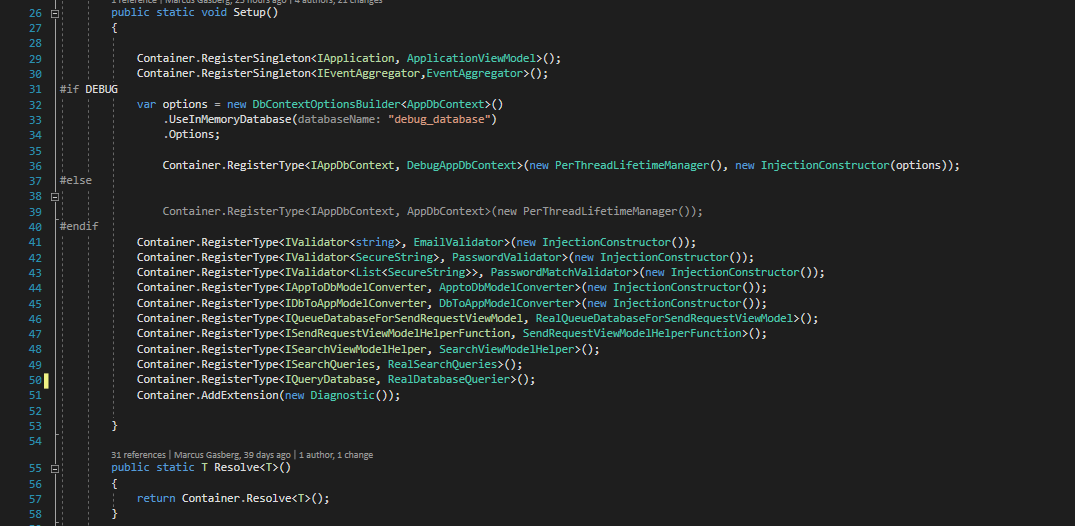
\includegraphics{Implementering/Graphic/IoCContainer.PNG}
    \caption{IoCContainer}
    \label{fig:IoCConatiner}
\end{figure}


\end{document}